\documentclass[a4paper,11pt,oneside,top=3cm,bottom=3cm,left=3.5cm,right=3.5cm,openright,reqno,table]{book}
\bibliographystyle{ieeetr}

\usepackage{packages}
\linespread{1.5}

\begin{document}
\begin{titlepage}
\changepage{}{}{}{-7.5 mm}{}{}{}{}{}

\begin{center}

\includegraphics [width=.15\columnwidth, angle=0]{unisa}\\ % height
\vspace{0.5cm}
{\LARGE \scshape Università degli Studi di Salerno}\\
\vspace{0.5cm}
{\Large Dipartimento di Informatica}\\
\vspace{0.1cm}
{\large Corso di Laurea Magistrale in Informatica}\\
\vspace{1.5cm}
{\Large \scshape Corso di Penetration Testing \\ and Ethical Hacking} \\
\vspace{4cm}
{\Huge \bfseries Penetration Testing Report: \\ \emph{Momentum: 1}} \\
\vspace{5cm}

\begin{minipage}[t]{7cm}
\flushleft
\textsc{Studente} \\
\textbf{Vincenzo Emanuele Martone} \\

\end{minipage}
\hfill
\begin{minipage}[t]{7cm}
\flushright
\textsc{Docente}

Prof. \textbf{Arcangelo Castiglione} \\
\end{minipage}

\vspace{1cm}

{\small Anno Accademico 2022-2023}
\end{center}

\end{titlepage}

\frontmatter

\cleardoublepage

\phantomsection
\addcontentsline{toc}{chapter}{Indice}
\tableofcontents
\clearpage

\cleardoublepage
\phantomsection
\addcontentsline{toc}{chapter}{Elenco delle figure}
\listoffigures
\mainmatter
\chapter{Penetration Testing Report}
\section{Executive Summary}
Per l'attività progettuale relativa al corso di \emph{Penetration Testing and Ethical Hacking} è stato svolto un processo di \emph{Penetration Testing} sulla macchina virtuale vulnerabile \emph{by-design} \emph{`Momentum: 1'}, disponibile sulla piattaforma \emph{VulnHub}. In assenza di particolari e specifiche informazioni relative all'asset da analizzare, è stato utilizzato un approccio di tipo \emph{Black Box}. Per svolgere l'analisi è stato configurato un opportuno ambiente simulato che consente un'interazione con l'asset, permettendo di esaminarlo e di rilevarne le vulnerabilità. In particolare, le vulnerabilità rilevate possono portare all'ottenimento del pieno controllo del sistema da parte di un attaccante che può assumere il ruolo di amministratore. Risulta, altresì, possibile per un attaccante rubare dati sensibili degli utenti del sito \emph{web}. Allo stato attuale, il livello di rischio complessivo associato all'asset risulta essere critico, tuttavia mediante alcuni accorgimenti, come la rimozione di dati sensibili dalle risorse pubbliche e l'implementazione di alcuni semplici controlli, è possibile abbassare sensibilmente il livello di rischio. 
\section{Engagement Highlights}
Dal momento che il processo di \emph{Penetration Testing} è stato svolto in un contesto puramente didattico, non è stato necessario definire particolari regole di ingaggio. 
\section{Vulnerability Report}
Nel corso del processo di \emph{Penetration Testing} sono state rilevate diverse vulnerabilità sfruttabili per compromettere vari aspetti del sistema. Di seguito è riportata una descrizione generale delle problematiche riscontrate:
\begin{itemize}
    \item \textbf{[Severity: Alta] Information Leakage del \emph{Web Server}}: presenza di una password usata per la decifratura di dati sensibili, all'interno di risorse pubblicamente accessibili mediante il \emph{Web Server}, che mette, altresì, a disposizione i dati sensibili cifrati. Tali dati rappresentano le credenziali di accesso di un utente del sistema;
    \item \textbf{[Severity: Alta] Information Leakage di un servizio in esecuzione all'interno del sistema}: presenza della password dell'amministratore del sistema nella memoria di un servizio accessibile anche da utenti non privilegiati;
    \item \textbf{[Severity: Media] Session Data Stealing}: possibilità di rubare i dati di sessione di un utente del \emph{Web Server} mediante l'iniezione di codice all'interno di una pagina;
    \item \textbf{[Serverity: Media] Navigabilità delle directory del \emph{Web Server}}: possibilità di navigare le directory del \emph{Web Server} mediante il \emph{Web Browser} al fine di visualizzarne il contenuto;
    \item \textbf{[Severity: Media] Errata configurazione del \emph{Web Server}}: assenza di attributi di controllo all'interno delle risposte del \emph{Web Server} volte alla protezione da alcuni tipi di attacchi noti. Il \emph{Web Server} lascia, inoltre, trapelare informazioni sul sistema;
    \item \textbf{[Severity: Media] Utilizzo di una versione non aggiornata del \emph{Web Server}};
    \item \textbf{[Severity: Bassa] Trapelamento del \emph{timestamp} del sistema}: ottenimento di informazioni sul \emph{timestamp} del sistema con eventuale possibilità di prevedere dati generati in maniera arbitraria dal sistema.
\end{itemize}
\section{Remediation Report}
Mediante vari accorgimenti risulta possibile rimuovere le vulnerabilità dal sistema evitando, in questo modo, tutti i rischi ad esse associate. Di seguito è riportata una descrizione generale delle operazioni consigliate:
\begin{itemize}
    \item Rimozione delle informazioni sensibili dalle risorse messe a disposizione dal \emph{Web Server};
    \item Implementazione di alcuni filtri per evitare l'iniezione di codice nelle pagine del sito \emph{Web};
    \item Riconfigurazione del \emph{Web Server} al fine di impedire la navigazione delle directory e di impostare opportuni attributi di sicurezza;
    \item Aggiornamento del \emph{Web Server} all'ultima versione stabile disponibile;
    \item Inibizione del trapelamento delle informazioni relative al \emph{timestamp} del sistema.
\end{itemize}
\section{Findings Summary}
Di seguito sono riportati i grafici relativi alle vulnerabilità identificate in rapporto alla severity. In particolare, l'aerogramma illustrato nella figura \ref{fig:aerogramma} ne mostra la percentuale, mentre l'ortogramma mostrato nella figura \ref{fig:istogramma} ne mostra il numero.
\begin{figure}[h]
    \centering
    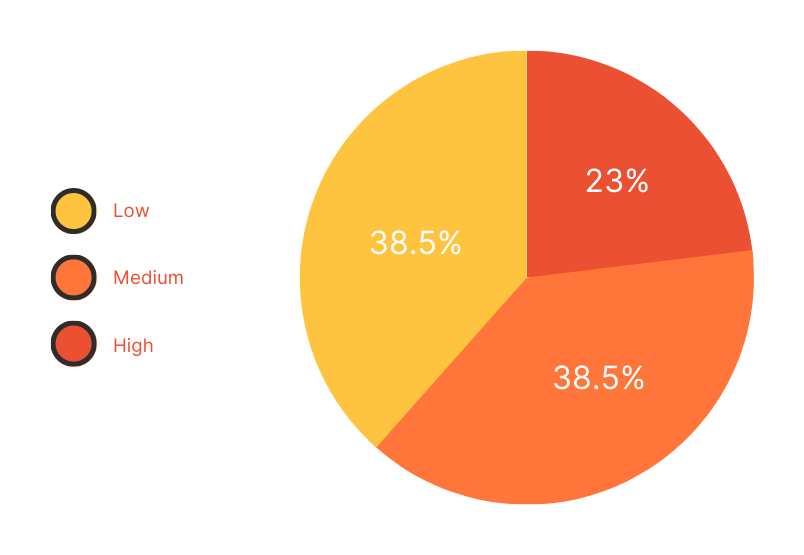
\includegraphics[scale=0.4]{capitoli/images/aerogramma.png}
    \caption{Aerogramma delle vulnerabilità rilevate}
    \label{fig:aerogramma}
\end{figure}

\begin{figure}[h]
    \centering
    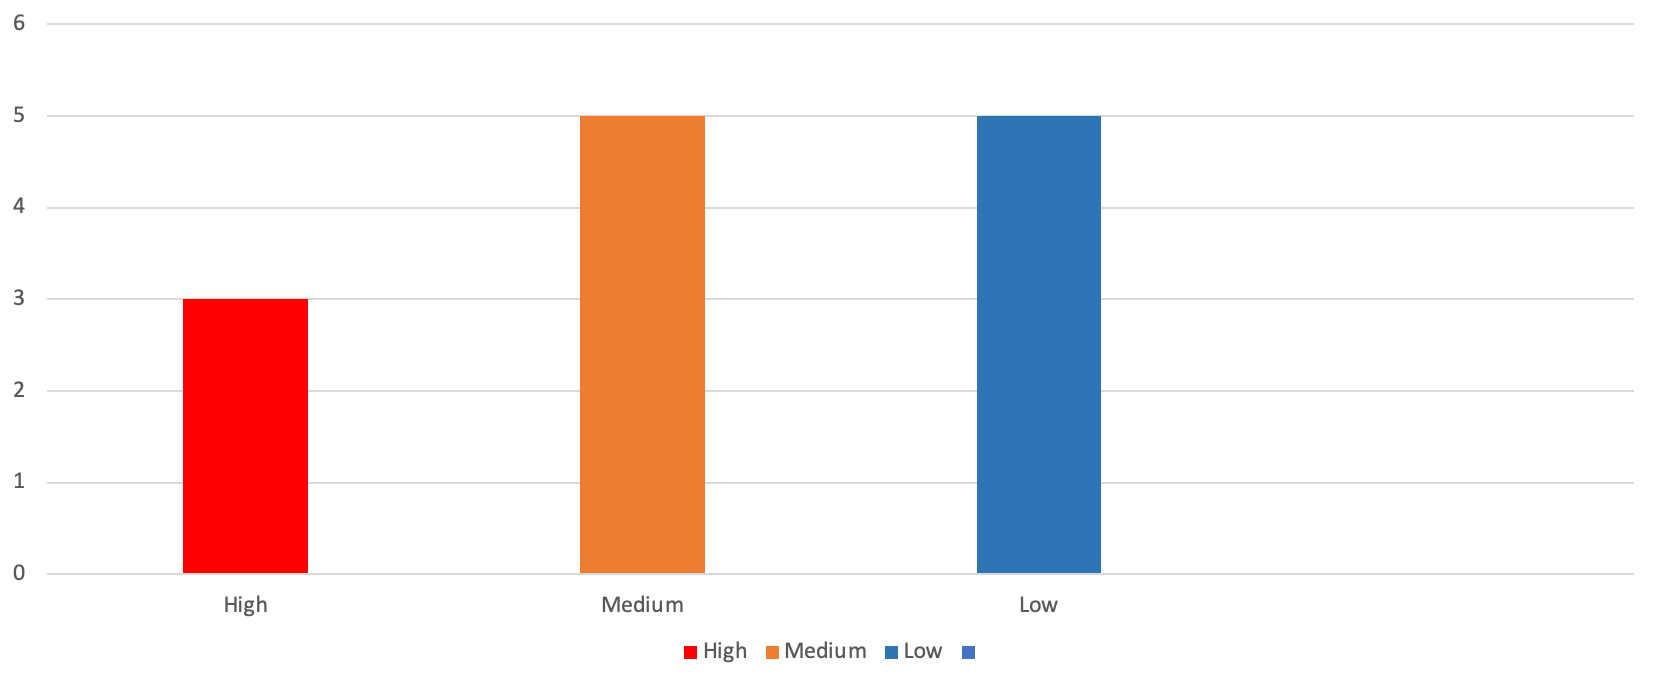
\includegraphics[scale=0.4]{capitoli/images/ortogramma.png}
    \caption{Ortogramma delle vulnerabilità rilevate}
    \label{fig:istogramma}
\end{figure}
\section{Detailed Summary}
Le vulnerabilità discusse sono state rilevate sia mediante l'utilizzo di specifici \emph{tool} che mediante tecniche di ricerca manuale. Complessivamente sono state rilevate 13 vulnerabilità e c'è stato un \emph{End of Life Detection} del \emph{Web Server}. 
\subsection{Vulnerabilità rilevate mediante i tool}
\subsubsection{OpenVAS}
\emph{OpenVAS} ha rilevato le seguenti due vulnerabilità aventi severity bassa:
\begin{itemize}
    \item \textbf{ICMP Timestamp Reply Information Disclosure};
    \item \textbf{TCP Timestamps Information Disclosure}.
\end{itemize}
Un report esaustivo relativo a tali vulnerabilità è riportato nel file \emph{`openvas-report.pdf'} reperibile nella directory \emph{`tools\_output'}.
\subsubsection{Nessus}
\emph{Nessus} ha rilevato le seguenti due vulnerabilità di severity media:
\begin{itemize}
    \item \textbf{Browsable Web Directories};
    \item \textbf{Web Application Potentially Vulnerable to Clickjacking}.
\end{itemize}
Un report esaustivo relativo a tali vulnerabilità è riportato nel file \emph{`nessus-web-all-ports-complex-report.pdf'} reperibile nella directory \emph{`tools\_output'}. A tal proposito, è doveroso sottolineare che \emph{Nessus} ha rilevato due falsi positivi: \emph{CGI Generic SSI Injection (HTTP headers)} e \emph{Web Application Information Disclosure}, che risulta opportuno ignorare nel corso della consultazione del report.
\subsubsection{OWASP ZAP}
\emph{OWASP ZAP} ha rilevato tre vulnerabilità aventi severity media e due vulnerabilità aventi severity bassa:
\begin{itemize}
    \item \textbf{Content Security Policy (CSP) Header Not Set};
    \item \textbf{Directory Browsing};
    \item \textbf{Missing Anti-clickjacking Header};
    \item \textbf{Server Leaks Version Information via "Server" HTTP Response Header Field};
    \item \textbf{X-Content-Type-Options Header Missing}.
\end{itemize}
Un report esaustivo relativo a tali vulnerabilità è riportato nel file \emph{`zap-report.html'} reperibile nella directory \emph{`tools\_output'}.

\subsubsection{Nikto 2}
\emph{Nikto 2} ha rilevato diverse vulnerabilità senza, tuttavia, fornire un livello di severity associato. Per alcune di queste vulnerabilità è stato, tuttavia, fornita la relativa \emph{CVE} che ha consentito l'identificazione della severity. Le vulnerabilità in questione sono le seguenti:
\begin{itemize}
    \item \textbf{The anti-clickjacking X-Frame-Options header is not present }: questa vulnerabilità è stata rilevata anche da altri tool che hanno assegnato una severity media;
    \item \textbf{The X-Content-Type-Options header is not set}: questa vulnerabilità è stata rilevata anche da altri tool che hanno assegnato una severity bassa;
    \item \textbf{Server may leak inodes via ETags (CVE-2003-1418)}: consultando il sito del \emph{NIST}, emerge che tale vulnerabilità ha una severity media \cite{inode}.
\end{itemize}
Il report delle vulnerabilità di \emph{Nikto} è riportato nel file \emph{`nikto2-report.html'} reperibile nella directory \emph{`tools\_output'}. Tra le vulnerabilità rilevate è possibile osservare una \emph{End Of Life detection} relativo alla versione di \emph{Apache 2.2.34}. 

\subsubsection{Paros Proxy}
\emph{Paros Proxy} ha rilevato tre vulnerabilità di cui due aventi severity media ed una avente severity bassa. Le vulnerabilità in questione sono le seguenti:
\begin{itemize}
    \item \textbf{Directory browsing};
    \item \textbf{Cross site scripting};
    \item \textbf{Private IP disclosure}.
\end{itemize}
Un report esaustivo relativo a tali vulnerabilità è riportato nel file \emph{`paros-report.htm'} reperibile nella directory \emph{`tools\_output'}. A tal proposito, è doveroso sottolineare che \emph{Paros Proxy} ha rilevato un falso positivi: \emph{Lotus Domino default files}, che che risulta opportuno ignorare nel corso della consultazione del report.

\subsection{Vulnerabilità rilevate mediante le tecniche manuali}
Le vulnerabilità aventi severity più elevata sono state rilevate mediante tecniche manuali di esplorazione dei servizi della macchina target. Di seguito è riportato un report dettagliato di tali vulnerabilità.

\subsubsection{Presenza di una password nel sorgente di una pagina \emph{Web}}
\begin{itemize}
    \item \textbf{Descrizione}: all'interno del file \emph{`main.js'} presente sul \emph{Web Server} vi è un commento contenente delle operazioni di decifratura che fanno uso della password in chiaro \emph{`SecretPassphraseMomentum'};
    \item \textbf{Modalità di individuazione}: la vulnerabilità è stata individuata durante un'operazione di \emph{browsing} delle directory del \emph{Web Server};
    \item \textbf{Rischi associati}: tale password può essere utilizzata per decifrare i dati inviati dal \emph{Web Server}. In particolare è possibile decifrare il contenuto di un cookie;
    \item \textbf{Severity}: Alta;
    \item \textbf{CWE di riferimento}: CWE-200 (Exposure of Sensitive Information to an Unauthorized Actor);
    \item \textbf{Soluzione}: rimuovere il commento dallo script \emph{`main.js'};
    \item \textbf{Riferimenti}: https://cwe.mitre.org/data/definitions/200.html
\end{itemize}

\subsubsection{Presenza di un cookie cifrato contenente la password di accesso al servizio \emph{SSH}}
\begin{itemize}
    \item \textbf{Descrizione}: quando l'utente visita la pagina \emph{`<WEB\_SERVER\_IP>/opus-details.php'}, il \emph{Web Server} gli invia un cookie che può essere decifrato con la password presente all'interno dello script \emph{`main.js'};
    \item \textbf{Modalità di individuazione}: la vulnerabilità è stata individuata durante la ricerca di un dato da decifrare con la password presente all'interno dello script \emph{`main.js'};
    \item \textbf{Rischi associati}: la decifratura di tale cookie porta alla scoperta di una stringa che rappresenta la password di accesso dell'utente \emph{`auxerre'} al servizio \emph{SSH} del sistema;
    \item \textbf{Severity}: Alta;
    \item \textbf{CWE di riferimento}: CWE-200 (Exposure of Sensitive Information to an Unauthorized Actor);
    \item \textbf{Soluzione}: rimuovere il cookie contenente la password di accesso al servizio \emph{SSH} e sostituirlo con uno cifrato utilizzando una password non reperibile;
    \item \textbf{Riferimenti}: https://cwe.mitre.org/data/definitions/200.html
\end{itemize}

\subsubsection{Presenza della password dell'utente \emph{root} all'interno dello storage di \emph{Redis}}
\begin{itemize}
    \item \textbf{Descrizione}: all'interno dello storage del \emph{key-value store `Redis'} è presente una chiave chiamata \emph{`rootkey'} alla quale è associata la password dell'utente \emph{root};
    \item \textbf{Modalità di individuazione}: la vulnerabilità è stata individuata durante la ricerca di un metodo per effettuare la \emph{privilege escalation} all'interno del sistema, dopo aver effettuato l'accesso con l'utente \emph{`auxerre'};
    \item \textbf{Rischi associati}: l'utilizzo di tale password permette ad un utente non privilegiato di accedere all'account \emph{root}, ottenendo, in questo modo, i massimi privilegi all'interno del sistema;
    \item \textbf{Severity}: Alta;
    \item \textbf{CWE di riferimento}: CWE-200 (Exposure of Sensitive Information to an Unauthorized Actor);
    \item \textbf{Soluzione}: rimuovere la chiave \emph{`rootpass'} all'interno dello storage di \emph{Redis};
    \item \textbf{Riferimenti}: https://cwe.mitre.org/data/definitions/200.html
\end{itemize}

\bibliography{bibliografia.bib}
\end{document}
